% This LaTeX was auto-generated from MATLAB code.
% To make changes, update the MATLAB code and export to LaTeX again.

\documentclass{article}

\usepackage[utf8]{inputenc}
\usepackage[T1]{fontenc}
\usepackage{lmodern}
\usepackage{graphicx}
\usepackage{color}
\usepackage{listings}
\usepackage{hyperref}
\usepackage{amsmath}
\usepackage{amsfonts}
\usepackage{epstopdf}
\usepackage[table]{xcolor}
\usepackage{matlab}

\sloppy
\epstopdfsetup{outdir=./}
\graphicspath{ {./AnimatedPlots_images/} }

\begin{document}

\matlabtitle{Example: Animated Plots}

\begin{par}
\begin{flushleft}
Here's an example of animated plots that you get when you plot stuff in a loop in a Live Script.
\end{flushleft}
\end{par}

\begin{matlabcode}
ax = axes;
axis(ax, [0, 2*pi, -1, 1])
hold(ax, "on")

for i = linspace(0, 2*pi)
    scatter(ax, i, cos(i), 'b')
    drawnow limitrate
end
\end{matlabcode}
\begin{center}
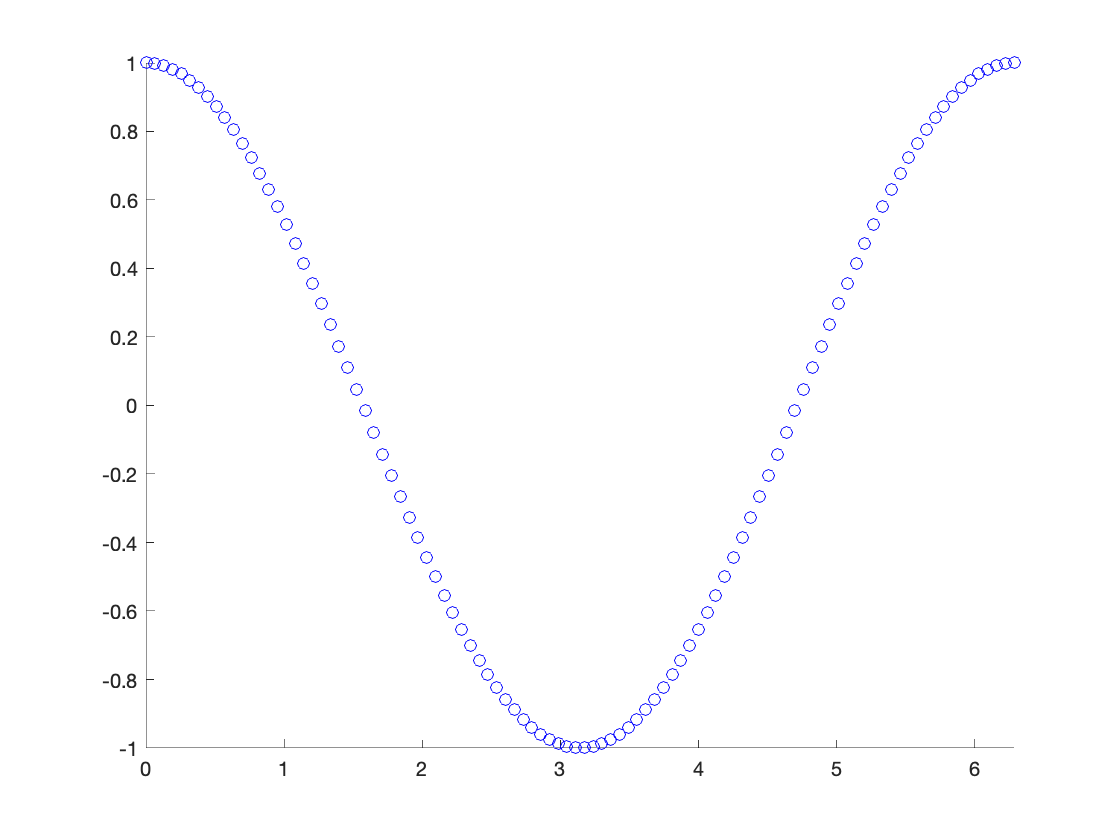
\includegraphics[width=\maxwidth{56.196688409433015em}]{figure_0.png}
\end{center}

\begin{par}
\begin{flushleft}
We'll try to figure out how to export those as animated GIFs or video files or something.
\end{flushleft}
\end{par}

\begin{par}
\begin{flushleft}
When you run the Live Script, it only does one pass through the sequence. How should we handle that?
\end{flushleft}
\end{par}

\end{document}
